\documentclass[margin=5mm]{standalone}
\usepackage{tikz}
\usetikzlibrary{patterns}
\definecolor{capri}{rgb}{0.0, 0.75, 1.0}
\definecolor{airforceblue}{rgb}{0.36, 0.54, 0.66}
\begin{document}
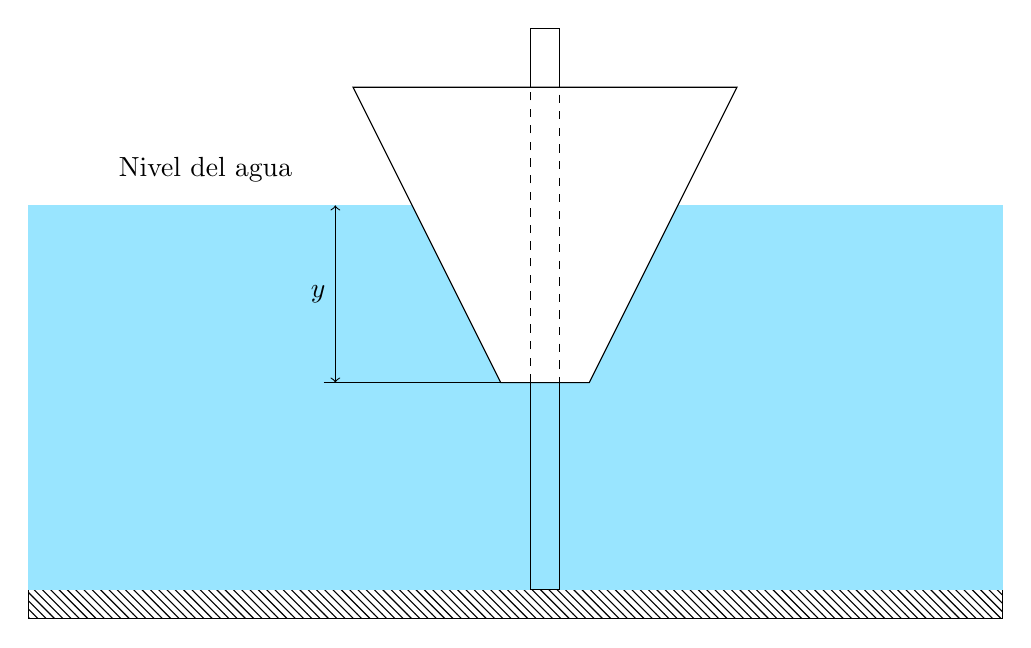
\begin{tikzpicture}[scale=1.5]
    \draw [pattern=north west lines] (-0.5, 0) rectangle (7.75, 0.25);
    \draw [fill, color=capri!40!white] (-0.5, 0.25) rectangle (7.75, 3.5);
    \draw (3.75, 0.25) rectangle (4, 2);
    \path [draw, fill=white] (3.5, 2) -- (4.25, 2) -- (5.5, 4.5) -- (2.25, 4.5) -- (3.5, 2) -- cycle;
    \draw [dashed] (3.75, 2) rectangle (4, 4.5);
    \draw (3.75, 4.5) rectangle (4, 5);
    \draw (2, 2) -- (3.75, 2);
    \draw [<->] (2.1, 2) -- (2.1, 3.5) node [left, midway] {$y$};
    \node at (1, 3.8) {Nivel del agua};
    
\end{tikzpicture}
\end{document}